\section{Produktübersicht}
\subsection{Systemarchitektur}

\begin{figure} [h]	
	\centering
	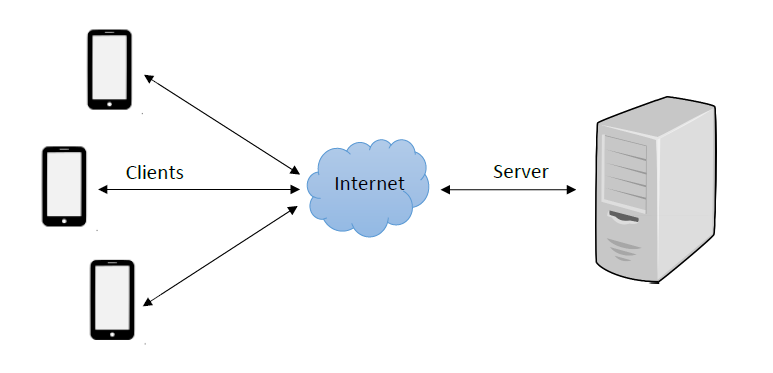
\includegraphics[scale = 0.8]{res/clientServerArchitektur.png}
\end{figure}

Aufgrund der Verknüpfung und des Informationsaustausches mehrere Mobiltelefone ohne konkrete Kenntnis 
voneinander, wird hier deshalb eine Client-Server-Architektur verwendet.

Es handelt sich um eine Client-Server Architektur, d.h. jeder Benutzer         
steht über einen zentralen Server in verbindung mit der Gruppe.
Der Server verwaltet die Gruppen, das Abbilden von Benutzernamen auf ID's
 
Das Client-Server-Modell oder -Architektur beschreibt das Prinzip der Kommunikation 
oder Interaktion zwischen zwei Teilnehmern in einem Netzwerk.
Diese Architektur unterscheidet zwischen der Anwender- bzw. Benutzerseite und der 
Anbieter- bzw. Dienstleisterseite. Der Anwender betreibt auf seinem Computer 
Anwendungsprogramme (Client), die die Ressourcen des Servers auf der Anbieterseite
zugreifen. Hier werden die Ressourcen zentral verwaltet, aufgeteilt und zur 
Verfügung gestellt.
Im Client-Server-Modell ist vorgesehen, dass immer der Client die Verbindung zum 
Server aufbaut. Nie umgekehrt. Der Client stellt eine Anfrage (Request). Der Server 
wertet die Anfrage aus und liefert eine Antwort bzw. die Daten zurück (Response oder Reply).
 


\subsection{Szenarien}
\subsection{Anwendungsfälle}
\subsubsection{Musskriterien}
\subsubsection{Wunschkriterien}